\documentclass{article}

% if you need to pass options to natbib, use, e.g.:
%     \PassOptionsToPackage{numbers, compress}{natbib}
% before loading neurips_2018

% ready for submission
% \usepackage{neurips_2018}

% to compile a preprint version, e.g., for submission to arXiv, add add the
% [preprint] option:
%     \usepackage[preprint]{neurips_2018}

% to compile a camera-ready version, add the [final] option, e.g.:
%     \usepackage[final]{neurips_2018}

% to avoid loading the natbib package, add option nonatbib:
%     \usepackage[nonatbib]{neurips_2018}

\usepackage[final,nonatbib]{neurips_2020}

\makeatletter
\renewcommand{\@noticestring}{}
\makeatother

\usepackage[utf8]{inputenc} % allow utf-8 input
\usepackage[T1]{fontenc}    % use 8-bit T1 fonts
\usepackage[hidelinks]{hyperref}       % hyperlinks
\usepackage{url}            % simple URL typesetting
\usepackage{booktabs}       % professional-quality tables
\usepackage{amsfonts}       % blackboard math symbols
\usepackage{nicefrac}       % compact symbols for 1/2, etc.
\usepackage{microtype}      % microtypography
\usepackage{xspace}
\usepackage{enumerate}
\usepackage{xcolor}
\usepackage{graphicx}

\newcommand{\nb}[1]{\textcolor{red}{#1}}
\urlstyle{rm}

\usepackage[backend=biber,sortcites=true,style=authoryear,maxbibnames=99]{biblatex}
\addbibresource{refs.bib}

\newcommand{\labeltrue}{\textsc{like}\xspace}
\newcommand{\labelfalse}{\textsc{dislike}\xspace}

\title{A straightforward method for evaluating performance of machine learning models for classification}

% The \author macro works with any number of authors. There are two commands
% used to separate the names and addresses of multiple authors: \And and \AND.
%
% Using \And between authors leaves it to LaTeX to determine where to break the
% lines. Using \AND forces a line break at that point. So, if LaTeX puts 3 of 4
% authors names on the first line, and the last on the second line, try using
% \AND instead of \And before the third author name.

\author{David J. T. Sumpter
  \today1\\
  Department of Information Technology, Uppsala University\\
  % examples of more authors
  % \And
  % Coauthor \\
  % Affiliation \\
  % Address \\
  % \texttt{email} \\
  % \AND
  % Coauthor \\
  % Affiliation \\
  % Address \\
  % \texttt{email} \\
  % \And
  % Coauthor \\
  % Affiliation \\
  % Address \\
  % \texttt{email} \\
  % \And
  % Coauthor \\
  % Affiliation \\
  % Address \\
  % \texttt{email} \\
}

\begin{document}
% \nipsfinalcopy is no longer used

\maketitle

\begin{abstract}
Imagine you have created an algorithm which assigns a score to a photograph based on how likely it is to contain a cat.  I propose the following steps to test performance of your model. First, you should set a threshold score such that when the algorithm is shown two randomly-chosen images --- one that has a score greater than the threshold (i.e. a picture labelled as containing a cat) and another from those pictures that really does contain a cat--- the probability that the image with the highest score is the one chosen from the set of real cat images is 50\%. This method thus sets a decision threshold, so that the set of positively labelled images are indistinguishable from the set of images which are truly positive. Once this threshold is established, as a second step, we measure performance by asking how often a randomly chosen picture from those labelled as containing a cat actually contains a cat. This measure is generally known as the recall, but we evaluate it specifically for the threshold chosen at the first step. The result is a single number measuring the performance of the algorithm. We explain, using an example, why this method avoids pitfalls inherent to, for example AUC, and is mathematically more pleasing and easier to explain than, for example, the F1-score.
\end{abstract}



\section{Article Summary}

The aim of this section is to describe the test in this paper as clearly as possible and to give an outline of the paper. The reader is encouraged to try the test on their own data set or on the artificial set we work with in this paper.

Imagine you have created an algorithm (a machine learning model) that assigns a score to some characteristics of an object to make predictions about whether it belongs to one of two classes (positive and negative). For example, the input might be a picture and the output whether or not the picture contains a cat. The scores are continuous values which are larger if your algorithm evaluates the object as more likely to belong to the positive class (i.e if it labels the image as more likely to contain a cat). Such a scoring system explicitly underlies, for example, logistic regression, the output of a neural network and discriminant analysis. Other, non-parametric machine learning methods, such as $k$-nearest neighbours, don't have an explicit score, but often have a parameter (e.g. $k$) which can be tuned in a way that mimics a threshold. 

\begin{figure}[p]
\centering
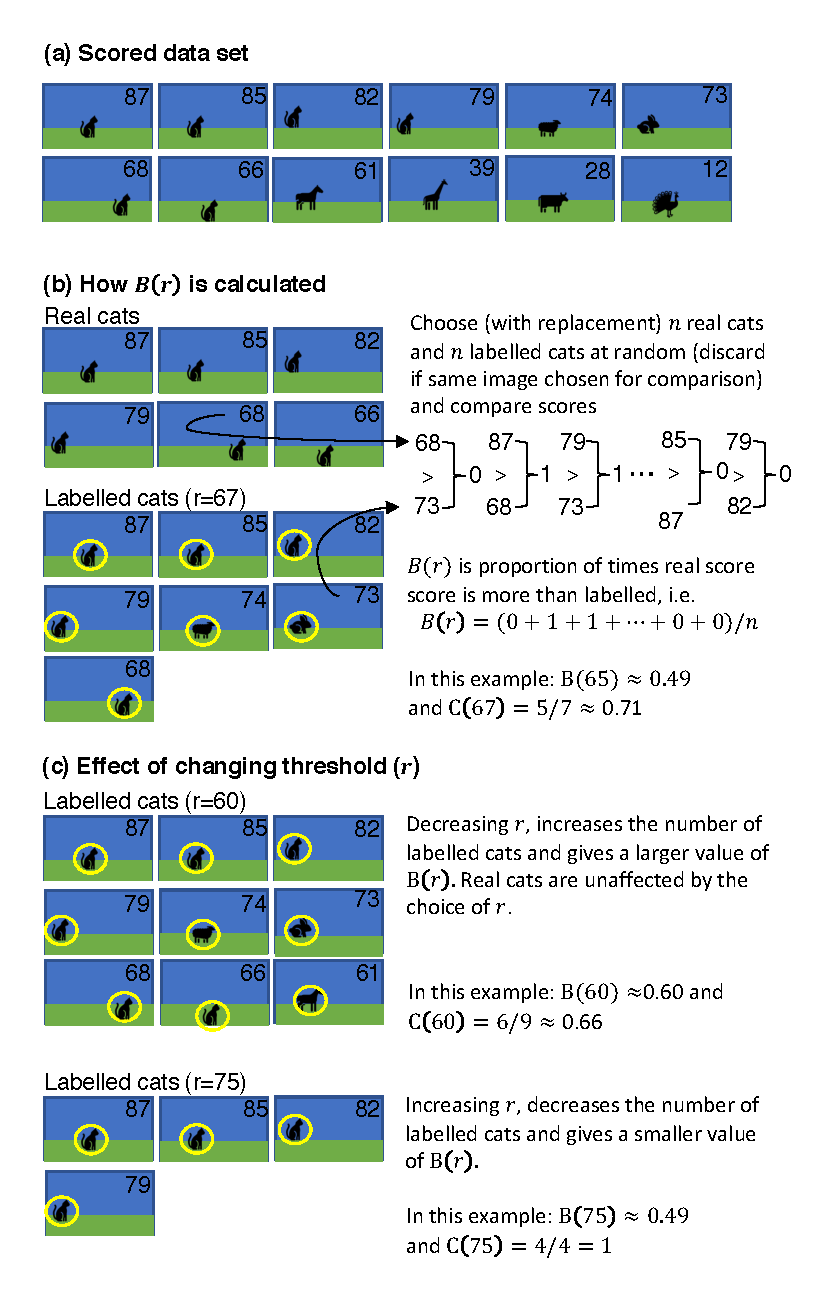
\includegraphics[scale=1]{Find Cats.pdf}
\caption{Illustration of the method described in this paper} \label{fig:methodill}
\end{figure}

The method then proceeds as follows. We start, in figure \ref{fig:methodill}a, with a data set in which every image is assigned a score. We now investigate what happens when we set a threshold score, $r$, above which we label the image as containing a cat (positive), below which we label the image as not containing a cat (negative). For any given threshold we compare those images  which we label as cats (given the threshold) with one containing real cats. Specifically, we choose (with replacement) $n$ real cats and $n$ labelled cats at random and compare scores (figure \ref{fig:methodill}b). Since some cats are in both sets, in some cases we will happen to pick the same two cats. If this occurs we pick two new cats for that comparison. This gives our measure $B(r)$, the probability a real cat scores more than a labelled cat for threshold $r$.

We then identify a specific threshold score, $r_b$, such that if we were to choose one image that the algorithm classifies as containing a cat and a second image that really does contain a cat, then the probability that the score of the image containing the cat is the largest of the two scores is 50\%.This is the value $r_b$ such that $B(r_b) \approx 0.5$. In the example, in figure \ref{fig:methodill}b this is $r=65$. A smaller threshold gives $B(r_b) > 0.5$ and a larger threshold gives $B(r_b) < 0.5$ (figure \ref{fig:methodill}c). We call $r_b$ the {\it indistinguishability threshold}: because  that that set comprised of false positives (FP) and true positives (TP) is indistinguishable from the set of TPs and true negatives (TN). If we pick (at random) two images from our data set, one which is labelled as a cat (when $r=r_b$) and the other that is known to contain a cat, then the probability that the algorithm will score assign the  image with the cat the highest score is one half. 

To measure the performance of your algorithm, simply calculate the proportion of images the algorithm classifies as containing a cat do actually contain a cat. We denote this $C(r_b$), recall at the indistinguishability threshold.

In this paper, I explain why the test described above is useful. I discuss one variant (for tuning in situations where not finding cats can be costly), look at its relation to other methods and also speculate how this method could be used in an improved boosting method. But otherwise the main results, now presented, are an argument for the test described above. To make this argument, this paper presents a series of three tests, which take us toward our final test, described above. Each of these three tests can be explained in plain English (or any other language) with reference to the application area (e.g finding cats). 

\section{Artificial data}

\begin{figure}[t]
\centering
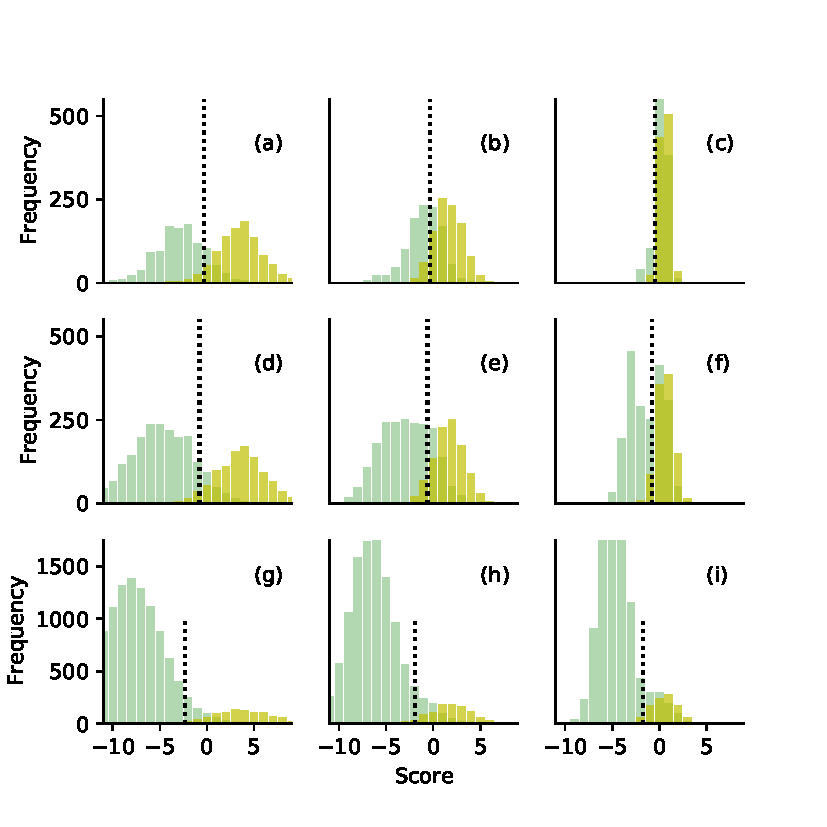
\includegraphics[scale=1]{Distribution.pdf}
\caption{The score distributions for the nine example data sets we look at here. Green are members of the negative class, yellow members of the positive class. The dotted line shows $r_b$, the solution $B(r)=1/2$ (see equation \ref{balanced})} \label{fig:Distribution}
\end{figure}

Throughout this article I use nine artificial data sets, as shown in figure \ref{fig:Distribution}. The positive class ($Y_i=1$) is created by first generating 1000 input values, $X_i$, with a mean $m_p=10$ and standard deviation $\sigma_p=2$. Similarly, the negative class ($Y_i=-1$) consists of 1000 'difficult' data points with values, $X_i$, which have mean scores (a,d,g) $m_n=5$; (b,e,h) $m_n=7$; (c,f,i) $m_n=9$ and (in all cases) standard deviation $\sigma_n=2$, along with (a,b,c) 10000; (d,e,f) 1000; (d,e,f) 100 'easy' data points, $X_i$, with mean 2 and standard deviation 2.  I then performed logistic regression on $X_i$ to predict $Y_i$ and calculated the log-likelihood for every individual point. These log-likelihoods are taken to be the scores, $S_i$, output by the model and are plotted in figure \ref{fig:Distribution}. 

\section{Area Under the Curve} 

{\bf How often does a member of the positive class score higher than a member of the negative class?} 

The sentence above summarises the nature of this test. We pick one member of the positive class at random and one member of the negative class at random and we will look to see which of them has the highest score. As a concrete example, imagine an algorithm is shown two images, one which contains a cat, another which does not. The task is to pick the image containing the cat. We call this probability 
\[
A = P(S_P>S_N)
\]
where $S_P$ is the score of a randomly chosen positive member and $S_N$ is the score of a randomly chosen negative member. This test tells us something useful about our model: the more often the algorithm passes the test, the better its performance. The value of $A$ can be measured directly, simply by randomly picking pairs of members of negative and positive classes and testing which scores higher. The test outcome is then the proportion of cases in which the positive member receives a higher value than the negative member.

We can also measure the paired comparison test over all our scores. Let $F_P(r)$ be the cumulative distribution of scores of the positive class, i.e. 
\begin{equation}
F_P(r) = P(S_P < r) = \int_{s=-\infty}^{r} f_P(r)  \label{eq:ScorefPr}
\end{equation}
where $f_P(r)$ is thus the probability density function of $S_P$. Likewise, we let $F_N(r)$ to be the cumulative distribution of scores the negative class, i.e. 
\begin{equation}
F_N(r) = P(S_N < r) = \int_{s=-\infty}^{r} f_N(r) \label{eq:ScorenPr}
\end{equation}
The value $A=P(S_P>S_N)$, can be written as the conditional probability distribution
\begin{equation}
A = \int_{r=-\infty}^{\infty} \int_{s=r}^{\infty}  f_N(r) \cdot  f_P(s) ds dr  \label{eq:SPgreaterSN}
\end{equation}
which is equivalent to
\begin{equation}
A = \int_{r=-\infty}^{\infty}  f_N(r)  \int_{s=r}^{\infty}  f_P(s) ds dr  = \int_{r=-\infty}^{\infty}  f_N(r) \cdot  \left(1 -  F_P(r) \right) dr \label{eq:SPgreaterSN2}
\end{equation}
We can use this equation to calculate $A$ by numerical integration. 

We can also use this formulation to note an important equivalence between our $A$ test and another commonly used measure of accuracy, namely, AUC (the area under the receiver operator curve). ROC curves plot the false positive rate against the true positive rate, as parametrised curves of $r$. Note that the true positive rate for a given threshold $r$ is given by $v(r)=1-F_P(r)$ and that the false positive rate for a given threshold $r$, is given by $u(r)=1-F_N(r)$. Then we see that
\[
A  =  \int_{r=-\infty}^{\infty} v(r) f_N(r) dr  
\]
which by change of variable gives
\begin{equation}
A  = \int_{u=0}^{1} v \left( u^{-1}(r) \right) du  \label{eq:AUCdef}
\end{equation}
where $u^{-1}(r)$ denotes the inverse of $u(r)$. Thus $A$ is also the area under the ROC curve (which is defined by the right hand side of equation \ref{eq:AUCdef}).

\begin{figure}[t]
\centering
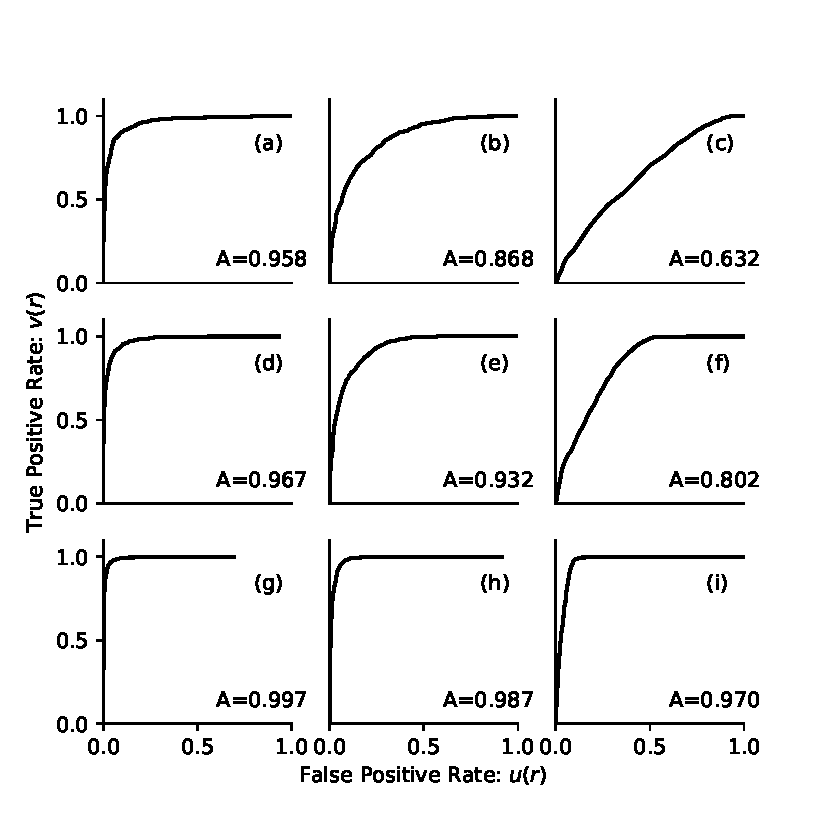
\includegraphics[scale=1]{AUC.pdf}
\caption{The area under the curve} \label{fig:AUC}
\end{figure}

The ROC curves are shown in figure \ref{fig:AUC} for our nine data sets. The area under these curves, which is also $A$, is shown as text within the figure. The value of $A$ is close to one when either the scores for the negative and positive class are typically different (e.g. for the score distributions shown in figure \ref{fig:Distribution} a, d and g) or there are a large proportion of 'easy' to score negative members (e.g. for the score distributions shown in figure \ref{fig:Distribution} h and i). 

These examples illustrate both the power and the limitation of $A$ as a measure. In the cases (a, d and g) where the score accurately distinguishes class members, $A$ reflects the fact it is more likely that the algorithm picks out the positive cases correctly. However, in the case where there is an overlap between the positive and 'difficult' negative class (e.g. cases c, h and i) then as we add more 'easy' cases (i.e. go from c to i) the accuracy of the model appears to increase, despite the fact that the difficult cases are equally difficult in each cases. We could see this as giving a possibility for `cheating': by adding more easier cases to our data set we can appear to be improving accuracy, as measured by $A$,

This is why we need to be very clear about what our test tells us: it tells us that if we pick one member of the positive class at random it has probability $A=0.965$ (in the case of figure \ref{fig:AUC}i) of having a higher score than one member of the negative class chosen at random. When there are a lot more 'easy'  to classify members of the negative class then a high value of $A$ is not surprising: most of the time we will randomly pick one of those members. So, in this case, an $A$ close to one tells us very little about how well our algorithm can distinguish more difficult cases. Our next two tests are designed to help us deal with such situations.

\section{Indistinguishability Threshold}

{\bf How often is a member of the positive class scored higher than a member that has been labelled positive?} 

We pick a random member of the positive class and we compare its score to the score of a random individual that has been labelled (predicted) positive. For example, in the cat labelling problem, we first pick randomly from all cats. We denote the score of this image as $S_P$. Then, for a given threshold $r$, we choose randomly from all the images with that score or above, irrespective of whether or not they contain a tumour. We denote this score of this image as $S_R$. We then calculate the probability 
\[
B(r) = P(S_P>S_R | S_R>r) 
\]
or, in words, the probability that a random member of the positive class scores higher than a random member of the class we have labelled as positive (i.e. has a score greater than $r$). 

Unlike the paired comparison of negatives and positives we made in the previous section, it is not immediately clear how comparing the positively labelled individuals to the positive class will help us. To gain some more intuition, let's think about what happens as we change the threshold $r$. When $r$ is very large then the positively labelled set will contain more positives than negatives, but very few members of either class. As a result $P(S_P>S_R | S_R>r)$ will be close to $0$. When $r$ is small (or negative), most images are labelled positive. Nearly all members of the positive class will be included in the positively labelled set, but so too will most members of the negative class (we will calculate an expression for this probability later in this section). Neither of these two situations is desirable. In the former, we will have a lot of false positive errors and very low recall (or sensitivity): a high proportion of those labelled positive will actually be negative. In the latter case, we will have a large proportion of false negatives but very high recall: most of those which are labelled positive are actually positive.

Can we use this probability to find a good balance? I suggest choosing $r_b$ such that
 \begin{equation}
B(r_b) = P(S_P>S_R | S_R>r_b) = 1/2 \label{balanced}
\end{equation}
This particular value of $r_b$ has a rather desirable property. It means that, as far as the classifier is concerned the images in the positive class are indistinguishable from those which we have labelled positive. If we pick a random member of the images we have classified as positive and a random member of the positives, these two images are equally likely to be classified as positive.

To understand why this is desirable, think about a situation where we have two separate test sets of images, $A$ and $B$, and we want to check whether or not they have a similar distribution of scores. A solution to this problem might be to pick members from both $A$ and $B$ at random and compare their scores. If (roughly) half of the time members of $A$ scored higher than members of $B$ we might say that the two groups are indistinguishable\footnote{There could still be differences between the distributions of the sets not identified by such a test. For example $A$ might have larger variance in scores than $B$}. This method is the basis of the sign test in statistics. In the same way,  by setting $r_b$ using equation \ref{balanced}, we are finding a threshold so that the positive class is indistinguishable from the set that is labelled positive. 

The vertical dotted lines in figure \ref{fig:Distribution} shows the value of $r_b$ for our nine example score distribution sets. For all nine distributions the lines give a reasonable separation between the scores, lying roughly half way between the `difficult' negative cases and the positive cases. The reason for this point of separation is chosen is that balancing the positive class and the positive predictions requires setting a threshold score above the scores of the `easy' negative cases, since inclusion of these cases will mean that $B(r)>1/2$. It is only when it becomes harder to distinguish the `difficult' negatives from the positives that we have $B(r)=1/2$. 

A common alternative to choosing $r=r_b$ is to instead choose $r$ such that
 \begin{equation}
P(S_P = r) = 1 - P(S_P=r) \label{standard}
\end{equation}
or, equivalently,
\begin{equation}
P(S_P = r) = 1/2 \label{standard2}
\end{equation}
where we define an underlying model which converts scores in to probabilities. For example, when the scores have been estimated by logistic regression then a natural choice is the logistic function
\[
P(S_P = r) = \frac{1}{1+\exp(r)} = 1/2
\] 
which gives $r=0$ as the threshold. Looking again at the distribution of scores in figure \ref{fig:Distribution}  we see that the size of the negative class shifts the distribution of the scores generated by the logistic regression to the right. This is undesirable, because it means that the algorithm will make more errors when easy to categorise cases are added to the data set.

The limitations of using equation \ref{standard2} to set a threshold are known, but often they are referred to as being ``caused by an unbalanced data set''. The implication is that too many members in the negative class have somehow misled us in to choosing a poor value of $r$. In my experience, students and even experienced practitioners, when confronted with this problem, either start to prune their data, removing `easy' members of the negative class, or oversample from the positive class in order to compensate. They might also draw an ROC curve and a Precision-Recall curve (see below) and try to justify, in an ad-hoc fashion, choosing a different value of the threshold $r$ on the basis of what they see in these curves.

It is not the data set that is imbalanced. It is rather our way of looking at it that is wrong! Specifically, it is the arbitrary choice of $r=0$ that is imbalanced (and wrong). While both of the two measures --- $A$ and $B(r)$ --- that we have looked at so far have sensible, method independent interpretations that give us a measure performance, this is not the case for equation \ref{standard}, which is simply the score for which the probability of receiving a positive label equals that of receiving a negative label. In logistic regression, the model is adjusting to account for the fact that negative cases are more likely than positive cases: negative cases are the more likely outcome and it requires more evidence to persuade us otherwise. But in an application where, for example, we are scanning for a medical condition, the number of negatives (be it 90\% or 99.99999\% of the population) should not influence how we decide that a case is likely to be positive. 

\begin{figure}[t]
\centering
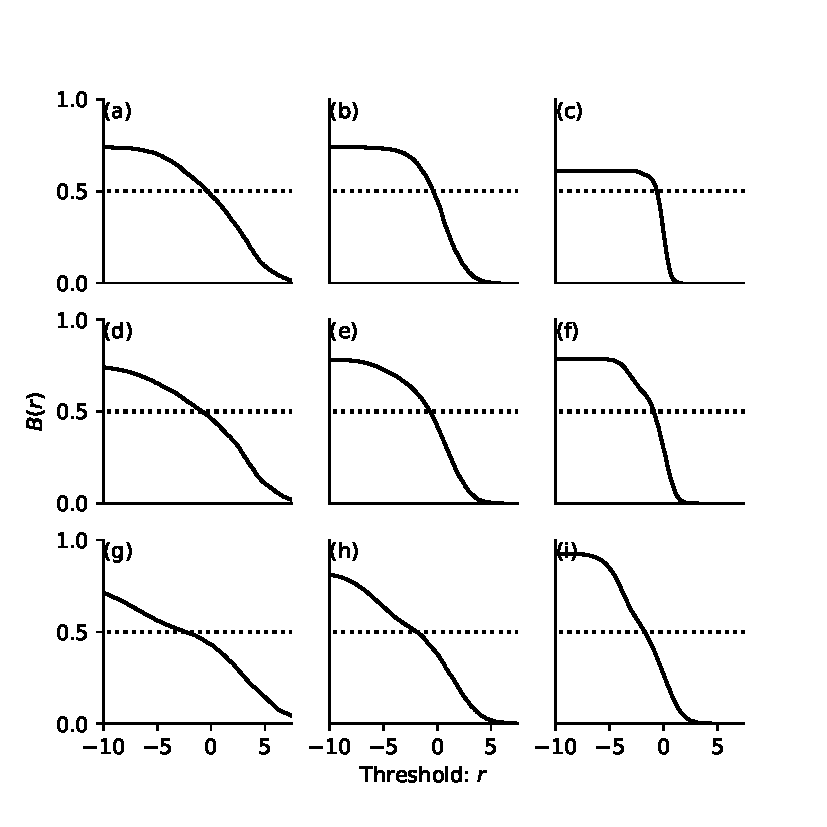
\includegraphics[scale=1]{Bplot.pdf}
\caption{Plot of $B(r)$ for our 9 example data sets. The dotted line is at $1/2$ indicates the value at which the model is balanced.}
\label{fig:Bplot}
\end{figure}

Neither $r_b$ nor $B(r)$ provide a measure of model performance, like $A$ does. Instead they are both measurements around which we can organise a rigorous evaluation of our model. We will look at how $B(r)$ can be used in the next section, but first we look at how it can be implemented. You can safely skip the rest of this section if you don't want to know the details yet, but it is worth pausing to look at figure \ref{fig:Bplot}, which shows how the value of $B(r)$ changes with $r$ and where it passes through $1/2$ for the nine data examples.

As with $A$ the pairwise nature of the test means it is straightforward to implement a randomised version of $B(r)$. For each value of $r$ we sample, with or without replacement, $n$ members of the positive class. Then we sample $n$ members from the set labelled positive when the threshold is greater than $r$. Pairwise comparison of the scores of these two sets gives $B(r)$ . This method becomes less reliable for large values of $r$, since the size of the positive labelled class becomes small and all the comparisons will be made to a small number of positively labelled images. 

Another way to calculate $B(r)$, following the AUC approach to estimating $A$, is by integration over the true positive rate, $y(r)$, and the false positive rate, $x(r)$. We now derive the appropriate integral. First, let $S_R$ be the score of a randomly chosen positive member. The probability the members has a score less than a randomly chosen member of the positive class with a score greater than $r$ is then written as $P(S_R<S_P | S_R>r)$. It is this probability we call $B(r)$. 

Our approach to finding an expression for $B(r)$ is to look separately at the case where $S_R$ is from a negative member and a positive member. We can use the law of total probability to give 
\begin{eqnarray}
B(r) &= &P(S_R < S_P | S_R>r) \nonumber \\
& = & P(S_R < S_P | S_{R} > r , R = + ) \cdot P( R = + | S_R > r )  \\
&&  + P(S_R < S_P | S_R>r, R= - ) \cdot P( R = - | S_R>r ) \label{eqn:totprobstep} 
\end{eqnarray}
where $+$ and $-$ are respectively the events that the chosen individuals are in the positive and negative classes. If an individual is chosen at random then 
\begin{equation}
P( R = + | S_R>r ) =   \frac{P v(r)}{N v(r) + P u(r)}  \mbox{ and }  P( R = - | S_R>r ) =   \frac{N u(r)}{N v(r) + P u(r)} \label{eqn:probbe}
\end{equation}
Furthermore,
\begin{eqnarray}
P(S_R < S_P | S_{R} > r ,  R = +   ) & = & \frac{P(S_R < S_P \cap S_{R} > r ,  R = +  )}{P(S_{R} > r ,  R = +  )} \nonumber \\
& = & \frac{\int_{t=r}^\infty \int_{s=t}^\infty f_P(t) f_P(s) dt}{\int_{t=r}^\infty f_P(t) dt} \nonumber \\
& = & \frac{\int_{t=r}^\infty f_P(t) v(t) dt}{v(r)} \label{eqn:posstep}
\end{eqnarray}
Since the derivative of $v(r)$ is equal to $-f_P(t)$ we can change variable to $v$ in the integral in the numerator to get
 \begin{eqnarray}
\int_{t=r}^\infty f_P(t) v(t) dt =  \int_{t=r}^\infty v(t) \left( -v'(t) \right) dt = \int_{v(r)}^\infty v(t) dv = \frac{v(r)^2}{2}
\end{eqnarray}
and thus simplify to get
\begin{equation}
P(S_R < S_P | S_{R} > r ,  R = +   ) = \frac{v(r)}{2} \label{eqn:posstepfinal}
\end{equation}
We can follow similar steps for the case that $R$ is negative to get,
\begin{equation}
P(S_R < S_P | S_{R} > r ,  R = -   ) = \frac{\int_{t=r}^\infty f_N(t) u(t) dt}{u(r)}  \label{eqn:negstep}
\end{equation}
Substituting \ref{eqn:probbe}, \ref{eqn:posstepfinal} and \ref{eqn:negstep} in to equation \ref{eqn:totprobstep} gives
\begin{equation}
B(r) = \frac{P v(r)^2/2 + N \int_{t=r}^\infty f_N(t) u(t) dt }{N v(r) + P u(r)} 
 \label{eqn:Bdef} 
\end{equation}
This equation is plotted as the black line in figure \ref{fig:Bplot}. We see that it goes towards a maximum when $r \rightarrow -\infty$, taking the value
\[
B(-\infty) = \frac{P/2 + N A}{N + P} 
\]
and decreases to zero as $r$ increases, so that $B(\infty) = 0$. The value $r_b$, the solution $B(r_b)=1/2$, is identified as the point in figure \ref{fig:Bplot} where $B(r)$ crosses the dotted line at $1/2$. This is also the value of $r_b$ plotted as the dotted line in figure \ref{fig:Bplot}. We will look in more detail at the function $B(r)$ in more detail in section \ref{sec:others} and compare it to other measures. 

We can think of $r_b$ as being the threshold value at which the model cannot distinguish between true positives and labelled positives. The algorithm cannot distinguish reality from its own labelling. We thus refer to $r_b$ as the threshold for indistinguishability.


\section{Recall at the Indistinguishability Threshold)}

How often is our positive labelling correct when reality and labelling are indistinguishibile? To answer this question, we define $C(r)$ to be the recall: the probability that an individual with a score greater than $r$ is in the positive class, i.e. $P(R = + | S_R > r)$ , or the probability that a positive labelling is made correctly.  Using Bayes law, we can rewrite recall in terms of false positive rate and true positive rate. Specifically,
\[
C(r) = P(R = + | S_R > r) = \frac{P(S_+ > r | R = + ) P(C = + )}{P(S_+ > r | R = + ) P(R = + ) + P(S_- > r | R = - ) P(R = - )}
\]
In this case, $P(R = + ) = P/(P+N)$ is the proportion of individuals in the positive class and $P(R = - ) = N/(P+N)$ is proportion in the negative class. Substituting $v(r)=P(S_+ > r | R = + )$ (true positive rate) and $u(r) = P(S_- > r | R = - )$  (false positive rate) gives
\begin{equation}
C(r) = P(R = + | S_C > r) = \frac{P v(r)}{P v(r) + N u(r)} \label{RecallP}
\end{equation}
When $N$ is much larger than $P$ then $v(r)$ has to be significantly larger than $u(r)$ for recall to have a large value. It is the ratio of true positives ($v(r)$) to all positives ($v(r)$ and $u(r)$), ighted by the frequency at which individuals are, respectively, positive and negative. 

\begin{figure}[t]
\centering
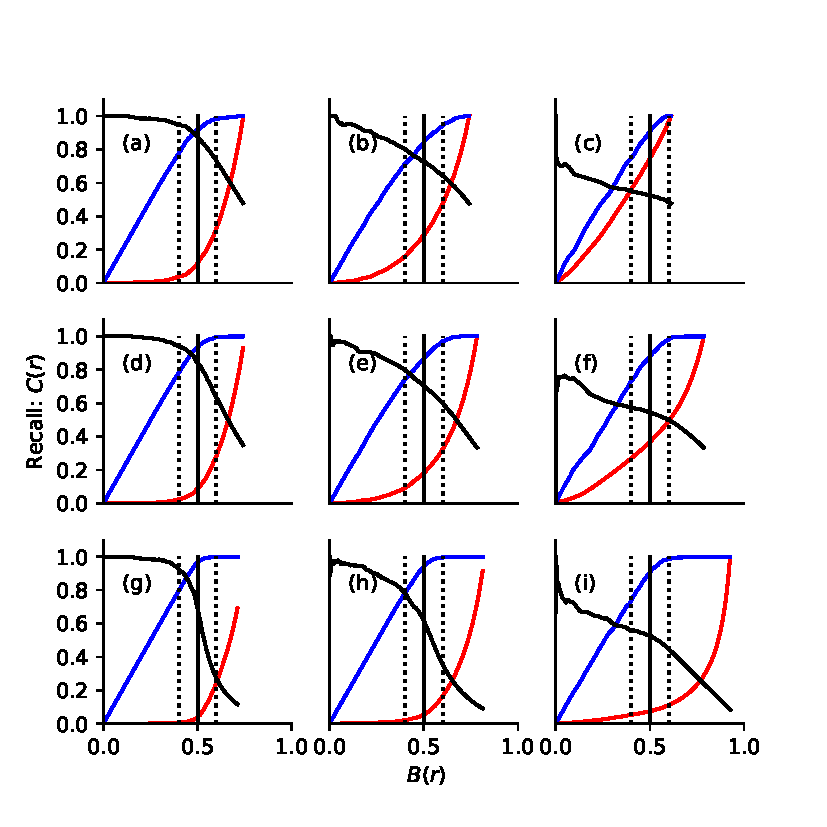
\includegraphics[scale=1]{Balance.pdf}
\caption{Plot of $B(r)$ against the recall $C(r)$ (blue), true positive rate $v(r)$ (yellow) and false positive rate $u(r)$ (green) for our 9 example data sets. These curves are parameterised by $r$. The numerical values are $C(r_b)=$ }
\label{fig:balance}
\end{figure}

Recall is widely used in assessing algorithm accuracy, in particular in plotting the precision recall curve. Our proposal is that recall should be primarily assessed when the algorithm is tuned so it cannot distinguish data it has classified as positive from data which truly is positive, i.e. we calculate $C(r_b)$. Evaluating this for the data in figure \ref{fig:Distribution} (a), (d) and (g) we get $C(r_b) \approx  0.85$. This could be considered a reasonably good performance: 85\% of the pictures the algorithm says are cats are in fact cats. For figure \ref{fig:Distribution}  (b), (e) and (h) we get $C(r_b) \approx 0.69$. This is not a great performance, but could be useable in certain applications: 69\% of the pictures the algorithm says are cats are in fact cats. Finally, for the data in figure \ref{fig:Distribution} \ref{fig:balance} (c), (f) and (i) we get $C(r_b) \approx  0.50$. This is poor performance, and is probably not very useful in most applications: only 50\% of the pictures the algorithm says are cats are in fact cats. 

We can now see why $C(r_b)$ is preferable measure of performance over $A$. When we calculated $A$, the value was highly dependent on the number of `easy' cases. This is not the case with $C(r_b)$. By evaluating recall when the algorithm cannot distinguish reality from its own labelling, we obtain a measure of performance that doesn't depend on the number of `easy' cases. As such, $r_b$ appears (in this case at least) to be a reasonable threshold to evaluate recall. It is theoretically motivated (in the previous section) and gives reasonable results. In section \ref{sec:others} we will compare $C(r_b)$ to other known metrics for measuring performance, but before we do this, we look at how we might be flexible about our choice of $r$. 


\section{Tuning false positive and true positive rates}

There are two further important questions we might ask. 
\begin{enumerate}
\item How	often is a member of the positive class detected by the test? This is the true positive rate ($v(r)$), yellow in figure \ref{fig:balance})
\item How often is a member of the negative class labelled positive by the test? This is the false positive rate ($u(r)$),green in figure \ref{fig:balance})
\end{enumerate}
Typically, one of these rates will be more important than another. For example, we might, in a medical screening task, accept a higher false positive rate in order to make sure all those who are positive for a condition are identified. In this case we set $r$ to be a smaller value so as to get a high true positive rate, but also (possibly) a high false positive rate.  In a targeted advertising task, where people who might be interested in a product should be identified, we might concentrate on having a lower false positive rate and accept a lower true positive rate, identifying only individuals who are very likely to be interested in the advertised product. In this case we set $r$ to a larger value. In general, there is no escaping from the fact that the measure of perfromance, and thus the choice of $r$, is informed by the application area.

An alternative here is to set an acceptable range for having a threshold which does not preserve the property that reality is indistinguishable from labelling. A rule of thumb  is 40/60. If, for example, we want to ensure a high level of true positives, we find $r_{60}$ by solving $B(r_{60})=0.6$, so that the probability a member classified as positive has a lower score than a truly positive member is 60\%. This is shown as the dotted lines in figure \ref{fig:balance} to the right of the solid line (at which $B(r_{b})=1/2$). Similarly, we can find $r_{40}$ by solving $B(r_{40})=0.4$, which is given to the left. Note that, while $B(r_{60})>B(r_b)>B(r_{40})$, the thresholds have the relationship $r_{60}<r_b<r_{40}$. A lower threshold leads to more true positives and more false positives. 

Figure \ref{fig:balance} shows $C(r)$ (black line) plotted against $r$ for our nine test data sets. Again, the way we built $B(r)$ allows us to explain in words what we are doing here. We can, for example, write about figure \ref{fig:balance}(e) that, "accepting a 60/40 imbalance in favour of positives our algorithm's predictions in favour of the positive class gave us a recall of $C()$, compared to $C(r_b)=$ at 50/50 balanced predictions." 

 The value in the top-right part of the figure is $C(r_b)$, the probability that a positive labelling is correct at balance. These values are strikingly similar for the data sets which have similar distributions for their 'difficult' negative cases. Specifically: figures \ref{fig:balance} 
As we have already seen, for $A$, a value near to $1/2$ implies the algorithm is no better than random and, as such, should not be used. A value near to $1$ indicates that the method is very accurate. Similarly, for $C(r_b)$, a value of 1 is an indication of accuracy, while the lowest possible accuracy is $P/(P+N)$, no more accurate than choosing a random individual. Note that, in figure \ref{fig:balance} (i), for example,  $P/(P+N)=1000/(1000+11000)=1/12$. So we could 'argue' that the algorithm is 6 times as accurate as random, since $C(r_b) \approx 6 P/(P+N)$. 

%The other way to address imbalances between true and false positive rates is to first assign a relative cost
% associated with each of them. So, for example, imagine a false negative is 10 times worse than a false positive, then a natural cost function 
%\begin{equation}
%10 (1-u(r)) + v(r)
%\end{equation}
%This is similar to the idea of bookmaker informedness \cite{powers2003recall}. It is the cost of making a mistake. For the data in \ref{fig:balance}(e) this cost is minimised when $r_{\mbox{min}}= -2.60$. This gives a balance of $B(r_{\mbox{min}})=0.646$ and a recall of $C(r_{\mbox{min}})=0.545$ (compared to $C(r_b)=0.734$ at balance).  We could write, that "by tuning our algorithm to favour true positives we reduce the recall fro $73.4$\% at balance, to $54.5$\%". In this particular example, the recall is now at a level comparable to that in figures \ref{fig:balance} (c), (f) and (i). We might think twice before putting such an algorithm in to production.


\section{Other performance measures}

\label{sec:others}

This section is a few notes about how $B(r)$ relates to some other measures of performance. To do this, I first break equation  $B(r)$ in to two components,
\begin{equation}
B(r) = B_+(r) + B_-(r)  \label{eqn:Bpmdef} 
\end{equation}
such that
\begin{equation}
B_+(r) =  \frac{P v(r)^2/2}{N v(r) + P u(r)} = \frac{1}{2} v(r) C(r)   \label{eq:poscomponentB}
\end{equation}
and 
\begin{equation}
B_-(r) = \frac{N \int_{t=r}^\infty f_N(t) u(t) dt }{N v(r) + P u(r)} 
 \label{eq:nehcomponentB}
\end{equation}
These terms are plotted in figure \ref{fig:Bplot2}. We now look at these two terms individually.

\begin{figure}[t]
\centering
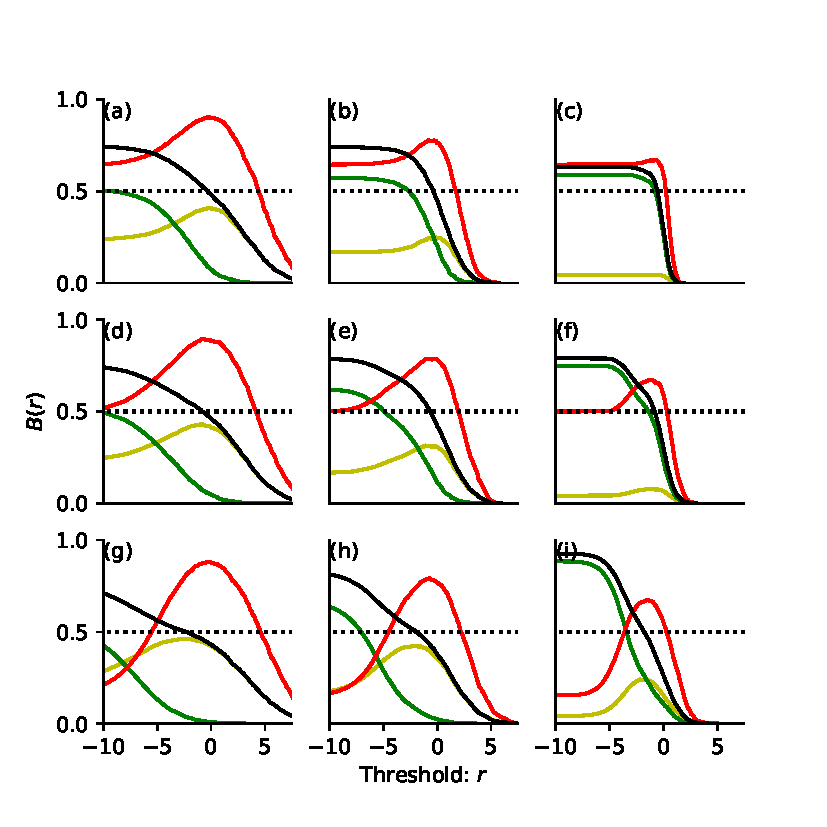
\includegraphics[scale=1]{Bplot2.pdf}
\caption{Plot of $B(r)$ for our 9 example data sets. The black line is $B(r)$. The dotted line at $1/2$ indicates the value at which the model is balanced. The yellow line is the component $B_+(r)$ (equation \ref{eq:poscomponentB}) and the green line is $B_-(r)$ (equation \ref{eq:negcomponentB}).  The red line is the $F_1(r)$ score (equation \ref{eq:F1}.}
\label{fig:Bplot2}
\end{figure}

Equation $B_+(r)$ is the recall multiplied by the true positive rate, divided by two. This is related to the the F1-score which is defined as,
\begin{equation}
F_1(r) =  \frac{2 C(r) v(r)}{C(r) + v(r)}   \label{eq:F1}
\end{equation}
In figure \ref{fig:Bplot2} we see that $F_1$ reaches a maximum at roughly the same point as which $B_+(r)$ is maximized.  Figure \ref{fig:Bplot2} shows that (with the exception of \ref{fig:Bplot2} g) the F1 score reaches a maximum at roughly the same point that $B(r)=1/2$. I have not derived the exact form of this relationship and it would be interesting to look at this in more detail, since F1 is seen as a standard test of model performance.

The measure $B_-(r)$ is similar to the integral which gives the area under the Precision-Recall curve, which is
\[
\int_{s=-\infty}^{\infty}  C(t) f_N(t) dt  \int_{s=-\infty}^{\infty}  \frac{P v(t)}{P v(t) + N u(t)} f_N(t) dt 
\]
The difference to $B_-(r)$, is that the integral includes the denominator. The term for $B_-(r)$ can also be thought of as a sort of $A(r)$, an AUC for those values with scores greater than $r$. Again, this needs to be looked at in more detail. My suspicion is that usage of area under Precision-Recall and F1 score just happen to approximate the (more principled) measure I describe here. But that is somewhat arrogant on my part, since I have not looked in detail at how these measured are justified.


\section{Summary}

The first test in this article, $A$, ---how often is a randomly chosen member of the positive class scored higher than randomly chosen member of the negative class?---is equivalent to calculating the AUC. In many applications, however, discerning between pairs of negative and positive cases might not be the most important challenge. Clinicians, for example, aren't usually presented with two people, one of whom they know is sick and one who is healthy, and asked to find the sick individual! Emphasising that $A$ answers a specific question about paired comparison makes its limitation clear: knowing $A$ tells us about paired comparisons between scores. It does not answer all questions we might have about the accuracy of our approach.

The second test, $B(r)$, doesn't, by itself, tell us about algorithm performance. It instead provides a principled way of deciding on the threshold, $r_b$, to choose for a decision. We tune our threshold, so that the set of pictures the algorithm labels as containing cats is indistinguishable from those which really do contain cats. In addition to laying the basis for our next test, one potentially useful application of this idea would be in boosting. If we fit a model first on all images, then we fit a new model on precisely the images with scores greater than $r_b$ then we may be able to iteratively improve the model fit.

The third test, $C(r_b)$, is the one I recommend for performance. We look at how often the positive labelling is correct when reality and labelling by the algorithm are indistinguishable. All tests of performance have a degree of arbitrariness, but the advantage of this one is that the threshold for the model is that the threshold is set on a single principle: that of indistinguishability. In our examples, this method avoided the limitations of $A$, where the addition of too many 'easy' cases inflated the area under the curve. 

No messing about with ROC or precision-recall curve. No need to make a confusion matrix. No need for all the bewildering array of 17 tests, with a total of 27 different names, which Wikipedia says can be performed on such problems. This paper has argued that the best way to measure performance is to calculate recall at a threshold set so that your algorithm can't distinguish between images it thinks there are cats in from those there really are cats in.  I look forward to seeing the wide use of this measure in the future. 

Test $C(r_b)$ is my final test (the test described above) and asks, when the algorithm can no longer distinguish labelled cats from real cats, how often is a randomly chosen member that is labelled positive actually a member of the positive class? This is generally known as the recall and is commonly used to evaluate model performance. I argue that recall should be interpreted primarily in the context of $B(r)$. Either we report a single value of recall when our threshold is set for indistinguishability as a measure of performance (i.e. $C(r_b)$) or if we decide that our algorithm is used in a way where the indistinguishability property does not hold (i.e. $B(r) \neq 1/2$) and then we report the value of $B(r)$ along with the recall, $C(r)$. Thresholds which don't obey indistinguishability can be justified for applications. But I argue that, as a guideline $B(r)$ should be between 40\% and 60\%.  I go on to look at some of the other tests on offer, including the precision-recall curve and the F1-score and discuss how $B(r_b)$ might be used to help improve model boosting. 



\end{document}

